
Este capítulo reúne a fundamentação teórica que sustenta o trabalho. Inicialmente, a Seção~\ref{sec:compiladores} apresenta os fundamentos de compiladores e suas fases, da análise léxica à geração de código objeto e à execução do código de máquina. A Seção~\ref{sec:engenharia-software} trata dos conceitos de engenharia de software que orientaram a construção do sistema: metodologias ágeis, testes automatizados, arquitetura em camadas, qualidade de código e o \textit{framework} adotado no \textit{back-end}. Em seguida, discutem-se os softwares educativos e as tecnologias de apoio à aprendizagem de programação. Por fim, a Seção~\ref{sec:trabalhos-relacionados} analisa os trabalhos relacionados, posicionando a solução proposta frente ao estado da arte.

\section{Compiladores}
\label{sec:compiladores}

Esta seção percorre os fundamentos de compiladores que embasam o núcleo de tradução implementado neste trabalho, desde a definição de compilador e de suas fases até a geração de código intermediário.

\subsection{Compiladores e seus Fundamentos}

Posto de forma simples, um compilador é um programa de computador que lê um programa escrito em uma linguagem fonte e o traduz para um programa equivalente em uma linguagem alvo. O modelo de compilação moderno é estruturado dividindo esse processo em duas partes fundamentais: a análise e a síntese. A fase de análise, frequentemente associada ao \textit{Front-End}, divide o programa fonte em suas partes constituintes e cria uma representação intermediária do mesmo. Por outro lado, a fase de síntese, ou \textit{Back-End}, constrói o programa alvo desejado a partir dessa representação intermediária gerada \cite{aho1995}.

\newpage
A Figura \ref{fig:fluxo_compilador} ilustra essa separação lógica e a progressão da transformação do código.

\begin{figure}[H]
    \centering
    \caption{Arquitetura de um compilador moderno.}
    \label{fig:fluxo_compilador}
    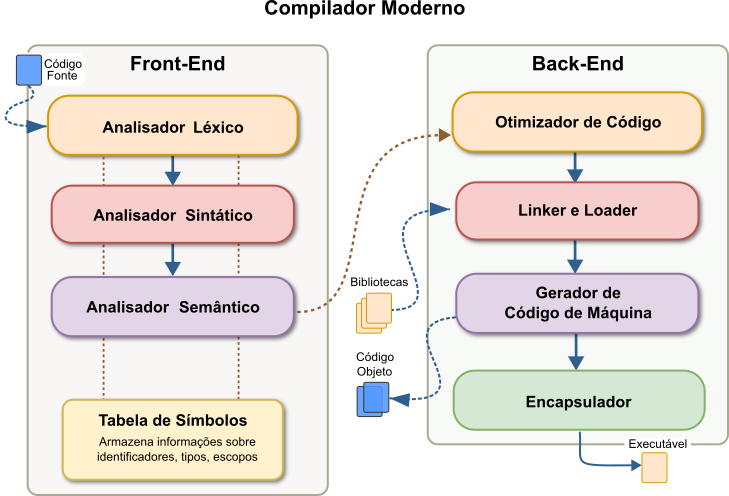
\includegraphics[width=0.8\textwidth]{Figuras/compiler.png}
    
    \legend{Fonte: \citeonline{alcantara2024}.}
\end{figure}

Conceitualmente, um compilador opera em fases sequenciais, cada uma das quais transforma o programa fonte de uma representação abstrata para outra. As primeiras fases formam o núcleo de análise e englobam a análise léxica, a análise sintática e a análise semântica. A partir daí, o fluxo avança para as etapas de geração de código intermediário, otimização e geração de código alvo. 

Interagindo com todas essas seis fases de compilação, encontra-se o gerenciamento da tabela de símbolos. Essa estrutura de dados é essencial para o compilador, pois atua registrando todos os identificadores usados no programa e coletando informações cruciais sobre seus atributos, permitindo rápida recuperação de escopos e validação semântica ao longo de todo o processo de tradução \cite{aho1995}.

% -------------------------------------------------------------------------------------------------
\subsection{O Modelo de Análise e Síntese (Fases da Compilação)}

O processo de compilação é tradicionalmente dividido em duas partes principais: a análise e a síntese.
A fase de análise, frequentemente chamada de \textit{front-end}, concentra-se em compreender o programa fonte dividindo o código em seus elementos constituintes para criar uma representação intermediária abstrata.
Em contrapartida, a fase de síntese, ou \textit{back-end}, foca em mapear e construir o programa alvo desejado a partir dessa representação intermediária.
A separação entre \textit{front-end} e \textit{back-end} atua como uma interface que facilita a adaptação e o suporte a múltiplas linguagens e arquiteturas \cite{cooper2012,price2001}.

Para dominar a complexidade da tradução de uma linguagem de alto nível, o fluxo geral é subdividido em módulos lógicos menores, conhecidos como fases, onde cada uma transforma a representação do programa para a etapa seguinte.
Em uma implementação prática, as atividades lógicas dessas fases podem ser agrupadas em ``passagens'' (\textit{passes}), otimizando o uso de memória durante o processo.
As principais fases que compõem o núcleo de um compilador são:

\begin{itemize}
    \item \textbf{Análise Léxica (\textit{Scanner}):} Constitui a primeira fase da compilação, fazendo a leitura do programa fonte caractere por caractere.
    Sua função é traduzir o texto para uma sequência de agrupamentos lógicos chamados de \textit{tokens}, ao mesmo tempo em que descarta caracteres não significativos, como espaços em branco e comentários.

    \item \textbf{Análise Sintática (\textit{Parser}):} Recebe a cadeia de \textit{tokens} do analisador léxico e verifica se a estrutura gramatical do programa está correta.
    O \textit{parser} agrupa os \textit{tokens} hierarquicamente, produzindo uma estrutura de dados conhecida como árvore de derivação ou árvore de sintaxe, seja através de estratégias \textit{top-down} (descendentes) ou \textit{bottom-up} (redutivas).

    \item \textbf{Análise Semântica:} Vai além da verificação estrutural sintática, realizando checagens para garantir que os componentes do programa fazem sentido e combinam-se de forma válida durante a execução.
    Um componente crítico desta fase é a verificação de tipos (\textit{type checking}), que assegura a consistência lógica do uso de variáveis e operadores.

    \item \textbf{Geração de Código Intermediário:} Após as análises, o compilador gera uma representação intermediária explícita que abstrai os detalhes específicos da máquina alvo, sendo o ``código de três endereços'' um de seus formatos clássicos.
    Essa etapa simplifica a implementação geral quebrando a barreira de complexidade entre a linguagem de alto nível e as instruções de baixo nível.

    \item \textbf{Otimização de Código:} Atua sobre o código intermediário com o objetivo de reescrevê-lo e melhorá-lo.
    Essa fase foca em reduzir o tempo global de execução e minimizar o espaço de memória consumido pelo programa compilado.

    \item \textbf{Geração de Código Objeto:} É a fase final de síntese, responsável por mapear o código intermediário para a linguagem alvo (código de máquina absoluto, relocável ou \textit{assembly}).
    Ela exige uma seleção cuidadosa das instruções nativas da máquina, das posições de memória e a alocação eficiente dos registradores.
\end{itemize}

Ao longo de todas as fases, o compilador interage ininterruptamente com dois módulos de suporte vitais: o gerenciador da \textbf{Tabela de Símbolos} e o \textbf{Atendimento a Erros}.
A tabela de símbolos registra os identificadores encontrados e armazena atributos essenciais (como escopo, tipo e métodos de transmissão de parâmetros) de maneira que permita uma recuperação extremamente rápida nas etapas posteriores.
Já o módulo de erros atua detectando falhas léxicas, sintáticas ou lógicas em todas as fases, utilizando mecanismos de recuperação que re-sincronizam o analisador e permitem que a compilação prossiga na tentativa de descobrir falhas adicionais no código fonte \cite{aho1995}.

% ----------------------------------------------------------------------------------------------

\subsection{A Análise Léxica e o Reconhecimento de \textit{Tokens}}

A análise léxica, frequentemente denominada \textit{scanner}, constitui a primeira fase do processo de compilação. A função primária deste módulo é realizar a leitura do programa fonte, caractere por caractere, e agrupá-los logicamente em unidades com significado gramatical, denominadas lexemas, conforme exemplificado na Figura \ref{fig:lexemas_nystrom}. 

\begin{figure}[htb]
    \centering
    \caption{Exemplificação de agrupamento de caracteres em lexemas.}
    \label{fig:lexemas_nystrom}
    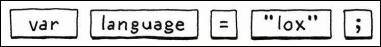
\includegraphics[width=0.8\textwidth]{Figuras/lex.png}
    \legend{Fonte: \citeonline[p. 43]{nystrom2021}.}
\end{figure}

Durante essa varredura, o analisador léxico também atua filtrando informações que não possuem relevância para as fases posteriores, descartando ativamente espaços em branco, tabulações e comentários inseridos pelo programador.

Neste contexto, é imprescindível estabelecer a distinção teórica entre dois conceitos fundamentais: o lexema e o \textit{token}. Um lexema é a sequência exata de caracteres no código-fonte que representa uma unidade léxica, ou seja, é a \textit{string} literal que foi digitada pelo usuário, como por exemplo a sequência ``123'' ou ``var''. Por outro lado, o \textit{token} é a representação lógica ou estrutura de dados gerada a partir desse lexema. Ele encapsula a classificação da unidade (sua classe ou categoria sintática, como identificador, palavra reservada ou operador) e, frequentemente, o valor original do lexema e sua posição no texto (linha e coluna) para auxiliar na emissão de erros sintáticos e semânticos \cite{nystrom2021,cooper2012}.

Para que o analisador léxico consiga identificar e classificar esses lexemas corretamente, a micro-sintaxe da linguagem de programação precisa ser formalmente descrita. Isso é realizado através de expressões regulares, que fornecem uma notação matemática concisa e poderosa para especificar a estrutura exata de cada tipo de \textit{token} (como, por exemplo, a regra que define que um identificador deve começar com uma letra seguida de letras ou dígitos). As expressões regulares descrevem conjuntos de cadeias de caracteres chamados de linguagens regulares, que figuram entre as linguagens mais simples na hierarquia das linguagens formais \cite{price2001}.

Embora as expressões regulares sejam excelentes para a especificação humana, o reconhecimento mecânico em tempo de execução exige um formalismo executável. Para a implementação computacional, as expressões regulares são traduzidas para autômatos finitos. Um autômato finito é uma máquina abstrata de transição de estados que atua como um reconhecedor. Ele processa a fita de entrada caractere por caractere, mudando de estado lógico; se, ao final da leitura de um lexema, o autômato atingir um estado de aceitação (estado final), o \textit{token} é validado e encaminhado para o analisador sintático.

O uso de autômatos finitos permite que a análise léxica seja extremamente eficiente, com custo de tempo linear em relação ao tamanho do código-fonte. Na prática, geradores de analisadores léxicos, como a clássica ferramenta \textit{Lex}, recebem as expressões regulares definidas pelo projetista da linguagem e geram automaticamente o código fonte de um autômato finito determinístico capaz de reconhecer os \textit{tokens} da linguagem de forma otimizada \cite{cooper2012}.

% -------------------------------------------------------------------------------------------------------------

\subsection{Estratégias de Análise Sintática: \textit{Top-Down} e \textit{Bottom-Up}}

A fase de análise sintática (ou \textit{parsing}) tem a responsabilidade central de determinar se a cadeia de \textit{tokens} fornecida pelo analisador léxico pode ser validamente gerada pela gramática formal da linguagem fonte. Para realizar essa verificação e construir a árvore de derivação, os compiladores adotam abordagens matemáticas que se enquadram majoritariamente em duas categorias fundamentais de algoritmos: a análise descendente (\textit{top-down}) e a análise ascendente ou redutiva (\textit{bottom-up}) \cite{aho1995,cooper2012}.

\subsubsection*{Análise Sintática Descendente (\textit{Top-Down})}
A estratégia descendente consiste na tentativa de construir a árvore de derivação a partir da sua raiz (o símbolo inicial da gramática) em direção às folhas (os \textit{tokens} terminais da cadeia de entrada). Em cada passo do processo, o analisador substitui o símbolo não-terminal mais à esquerda por um de seus lados direitos correspondentes nas regras de produção, realizando o que se denomina rigorosamente como uma derivação mais à esquerda (\textit{leftmost derivation}).

Os analisadores \textit{top-down} dividem-se tradicionalmente em preditivos tabulares (como o algoritmo LL(1)) e recursivos descendentes. A técnica de descida recursiva é amplamente utilizada em compiladores de produção modernos em virtude de sua elegância, facilidade de codificação manual e excelente capacidade de detectar e relatar erros de sintaxe. Contudo, para que um analisador descendente funcione de maneira eficiente e evite o custoso retrocesso (\textit{backtracking}), a gramática subjacente da linguagem deve atender a restrições estritas. Especificamente, a gramática não pode conter recursividade à esquerda e deve estar fatorada à esquerda, de modo que o próximo \textit{token} da entrada seja suficiente para guiar univocamente o analisador na escolha da produção correta \cite{nystrom2021,price2001}.

\subsubsection*{Análise Sintática Ascendente ou Redutiva (\textit{Bottom-Up})}
Em contrapartida à técnica anterior, a análise ascendente processa a estrutura do programa de baixo para cima, iniciando a construção da árvore a partir das folhas (os \textit{tokens} fornecidos pelo \textit{scanner}) e trabalhando estruturalmente em direção à raiz. 

A denominação ``redutiva'' deve-se à natureza do processo: o analisador busca identificar uma sequência de símbolos na pilha que corresponda exatamente ao lado direito de uma regra de produção (o \textit{handle}) e a substitui (reduz) pelo símbolo não-terminal correspondente ao lado esquerdo daquela regra. Esse mecanismo iterativo constrói sistematicamente uma derivação mais à direita ao reverso.

A família mais proeminente e poderosa de analisadores \textit{bottom-up} é a dos analisadores da classe LR (como SLR, LALR e o Canônico), que operam através de uma arquitetura do tipo empilha-reduz (\textit{shift-reduce}) orientada por tabelas de transição de estados. Ao contrário da abordagem descendente, os analisadores \textit{bottom-up} não impõem a restrição de ausência de recursão à esquerda, acomodando e processando com eficiência tanto a recursividade à direita quanto à esquerda. Ademais, são capazes de reconhecer virtualmente todas as construções sintáticas que podem ser descritas por gramáticas livres de contexto \cite{aho1995}. 

Entretanto, devido à enorme complexidade matemática requerida para a construção manual das tabelas de transição de estados LR, esses analisadores não costumam ser codificados à mão; ao invés disso, recorre-se a geradores automáticos de analisadores sintáticos, como a clássica ferramenta YACC, que produzem o código-fonte do \textit{parser} a partir de uma especificação gramatical \cite{cooper2012}.

% ---------------------------------------------------
\subsection{Análise Semântica e Verificação de Tipos}

Esta seção apresenta os fundamentos da análise semântica e da verificação de tipos, consolidando os conceitos e definições propostos por \citeonline{aho1995}, \citeonline{cooper2012}, \citeonline{price2001} e \citeonline{nystrom2021}.

Uma vez que a estrutura gramatical do código é validada pela análise sintática, o processo de compilação evolui para a fase semântica. O objetivo central aqui é garantir que as construções do programa, embora sintaticamente corretas, possuam coerência lógica para a futura execução. Enquanto o \textit{parser} se limita a verificar se a ``forma'' do código respeita as regras da linguagem, o analisador semântico atua como um inspetor que examina o significado das combinações entre os elementos do programa. Um dos pilares desse estágio é a resolução de nomes (ou amarrações), procedimento no qual o compilador mapeia cada identificador à sua declaração correspondente, respeitando as regras de escopo \cite{aho1995,cooper2012}.

A verificação de tipos constitui outro componente vital da análise semântica. Utilizando a árvore de derivação e as informações armazenadas na tabela de símbolos, o compilador checa se os operadores estão sendo aplicados a operandos compatíveis. Durante essa inspeção, o sistema infere os tipos das expressões e detecta interpretações de valores que seriam semanticamente inválidas. Caso a linguagem permita, o analisador também pode aplicar coerções, que são conversões implícitas de tipos (como transformar um inteiro em ponto flutuante) para viabilizar operações entre tipos distintos \cite{price2001,nystrom2021}.

\subsubsection*{Tipos de Erros Semânticos}

Diferente dos erros de sintaxe, as falhas semânticas ocorrem em códigos que possuem uma estrutura gramatical perfeita, mas que violam as regras de contexto ou significado da linguagem. O foco do tratamento de erros nesta fase é capturar inconsistências lógicas, destacando-se:

\begin{itemize}
    \item \textbf{Incompatibilidade de Tipos:} Manifesta-se quando um operador é utilizado com operandos cujos tipos não podem interagir entre si, seja por falta de suporte da linguagem ou por ausência de regras de conversão. Um caso típico em linguagens fortemente tipadas é a tentativa de realizar operações aritméticas entre textos (\textit{strings}) e valores lógicos (booleanos).
    
    \item \textbf{Identificadores Não Declarados e Violações de Escopo:} Este erro surge quando o programa tenta acessar uma variável, função ou objeto que não foi definido ou que não está visível no bloco de código atual. Um exemplo comum é a tentativa de utilizar uma variável local fora dos limites do seu escopo de definição.
    
    \item \textbf{Inconsistências de Aridade e Estruturais:} Refere-se a falhas na conformidade numérica de elementos. Isso inclui chamadas de funções com um número de parâmetros diferente do que foi estabelecido na assinatura original, ou o acesso a um \textit{array} utilizando um número de dimensões que não condiz com sua declaração \cite{aho1995}.
\end{itemize}

% -------------------------------------------------------------------------------------------------------------
\subsection{Geração de Código Intermediário}

A geração de código intermediário atua como um elo estrutural entre as fases de análise (\textit{front-end}) e síntese (\textit{back-end}) de um compilador. Após a verificação estrutural e semântica do código fonte, o compilador normalmente gera uma representação intermediária explícita, cujo formato é projetado para ser largamente independente das especificidades da linguagem fonte e da arquitetura da máquina alvo. A principal vantagem dessa estratégia em múltiplos passos é resolver, de maneira gradativa, a barreira de complexidade existente na conversão direta de comandos de alto nível para instruções de baixo nível. Ademais, essa etapa viabiliza a otimização de código e facilita a portabilidade, permitindo que a mesma representação interna seja traduzida para diversas arquiteturas diferentes \cite{cooper2012,price2001}.

Dentre as formas de representação linear utilizadas na literatura, destaca-se o uso do código de três endereços, que se assemelha a uma linguagem de montagem (\textit{assembly}) genérica e abstrata. Nesta notação, as expressões matemáticas e lógicas são desmembradas em instruções elementares que possuem, no máximo, três operandos. A grande distinção teórica entre o código intermediário e o código objeto final reside no fato de que o intermediário se abstém de especificar detalhes físicos de \textit{hardware}, como os registradores exatos e as posições absolutas de memória a serem alocadas \cite{nystrom2021}.

Para ilustrar o mecanismo, uma instrução aritmética convencional de atribuição, tal como \texttt{A := X + Y * Z}, seria mapeada em instruções \textit{pseudo-assembly} mais simples, por meio da criação automática de variáveis temporárias pelo compilador. O fluxo de código de três endereços resultante desta operação seria composto por passos sequenciais lógicos:
\begin{enumerate}
    \item \texttt{T1 := Y * Z}
    \item \texttt{T2 := X + T1}
    \item \texttt{A := T2}
\end{enumerate}

\subsubsection*{Método de Geração Dirigida pela Sintaxe}

Para que essa conversão ocorra de forma automatizada e correta, os compiladores comumente empregam a técnica denominada \textbf{tradução dirigida pela sintaxe}. Esse método estende os conceitos matemáticos das gramáticas livres de contexto, permitindo a associação direta de atributos aos símbolos gramaticais e a vinculação de ações semânticas específicas às regras de produção.

Na prática, isso significa que a geração de código pode ocorrer concomitantemente com a fase de análise sintática. À medida que o analisador (\textit{parser}) agrupa as unidades léxicas e reconhece uma construção gramatical válida, ele executa em paralelo a ação semântica correspondente a essa regra. Essa execução processa os atributos passados pelos nós filhos da árvore gramatical e sintetiza as informações, permitindo a emissão gradativa e ordenada dos trechos de código intermediário \cite{cooper2012}.

%--------------------------------------------------------------------------------------------------------------
\subsection{Otimização de Código e Eficiência Computacional}

Situada geralmente como a etapa intermediária do processo de compilação, a otimização visa refinar a representação interna do programa para torná-la mais performática. Esse aprimoramento busca não apenas acelerar a execução e reduzir o consumo de memória, mas também, em contextos tecnológicos modernos, diminuir o gasto energético do hardware. Durante esse estágio, o compilador substitui instruções genéricas por variantes mais ágeis e semanticamente equivalentes. Um exemplo clássico é o dobramento de constantes (\textit{constant folding}), que antecipa cálculos de valores fixos para o tempo de compilação, evitando que sejam processados repetidamente durante a execução \cite{aho1995,cooper2012}.

Para que uma técnica de otimização seja considerada válida, ela deve respeitar dois pilares fundamentais: a integridade (segurança) e a utilidade (rentabilidade). O princípio da segurança exige que qualquer modificação preserve o comportamento original do algoritmo, garantindo que o resultado final do programa não seja alterado. Já o princípio da rentabilidade assegura que a mudança estrutural resulte em um ganho de desempenho real e mensurável, justificando o tempo adicional despendido pelo compilador para realizar tal transformação \cite{price2001}.

Quanto à sua abrangência, o processo de otimização opera em diferentes níveis de profundidade, sendo categorizado em quatro escopos principais:

\begin{itemize}
    \item \textbf{Otimização Local:} Concentra-se na análise de blocos básicos, que são sequências de instruções sem desvios internos. Nesse nível, é comum o uso de Grafos Acíclicos Dirigidos (GADs) para identificar e remover subexpressões redundantes e otimizar o uso de variáveis locais.
    
    \item \textbf{Otimização Regional:} Estende a análise para grupos de blocos básicos, focando prioritariamente em laços de repetição (\textit{loops}). Como a maior parte do tempo de execução de um software costuma ocorrer dentro desses ciclos, melhorias aplicadas aqui geram impactos significativos no desempenho global.
    
    \item \textbf{Otimização Global (Intraprocedural):} Examina o contexto completo de uma função ou procedimento. Através de análises detalhadas de fluxo de dados, o compilador consegue identificar oportunidades de melhoria que não seriam visíveis em uma inspeção puramente local.
    
    \item \textbf{Otimização Interprocedural:} Atua de forma macro, atravessando as fronteiras entre os diferentes módulos e funções do programa. Isso possibilita técnicas agressivas como a substituição em linha (\textit{inlining}), onde o corpo de uma função é inserido diretamente no local da chamada, eliminando os custos computacionais associados ao desvio de execução e troca de contexto \cite{cooper2012}.
\end{itemize}

De maneira geral, a maioria das rotinas de otimização ocorre em duas fases complementares: primeiro, uma análise estática para mapear o fluxo de controle e dependências; segundo, a transformação sintática que efetivamente reescreve o código. Entre as manobras mais frequentes, destacam-se a eliminação de código morto (instruções inacessíveis), o deslocamento de cálculos para fora de laços e a simplificação de redundâncias aritméticas \cite{aho1995}.

\subsection{Geração de Código Objeto e Mapeamento de Arquitetura}

A fase de geração de código objeto (ou geração de código de máquina) constitui a etapa final do processo de compilação, englobando as atividades finais do \textit{back-end}. O principal objetivo desta fase é mapear a representação intermediária otimizada para a linguagem nativa da máquina alvo, garantindo que o código gerado seja logicamente correto, faça uso efetivo dos recursos de \textit{hardware} disponíveis e execute de forma altamente eficiente \cite{aho1995}.

Um dos maiores desafios enfrentados na geração de código objeto advém da diversidade arquitetônica dos processadores. Cada família de processadores (como as arquiteturas x86, ARM ou SPARC) dispõe de um conjunto próprio de instruções de máquina, também conhecido como Arquitetura do Conjunto de Instruções (ISA - \textit{Instruction Set Architecture}). Isso implica que as operações de baixo nível e suas respectivas codificações binárias diferem radicalmente de um computador para outro \cite{cooper2012}.

Para transpor essa barreira e evitar a necessidade de se construir um compilador inteiramente novo para cada arquitetura de \textit{hardware} existente, os compiladores modernos adotam o princípio da \textit{retargetabilidade} (capacidade de redirecionamento). Essa estratégia é viabilizada pelo uso do código intermediário: o \textit{front-end} atua de forma independente de máquina para gerar a representação intermediária, permitindo que a adaptação para um novo computador exija apenas a reescrita ou a substituição do módulo gerador de código (\textit{back-end}) \cite{aho1995,cooper2012}.

O processo de geração de código específico para uma máquina baseia-se fortemente em duas atividades interligadas: a seleção de instruções e a alocação de registradores. A seleção de instruções atua como um reconhecedor de padrões que analisa a árvore ou a sequência linear do código intermediário e seleciona a sequência exata de operações na ISA do processador capaz de implementar aquele comportamento com o menor custo de execução possível. Em paralelo, a alocação de registradores gerencia o escasso conjunto de registradores físicos da Unidade Central de Processamento (UCP), decidindo quais valores em tempo de execução serão mantidos nestes componentes de altíssima velocidade e quais precisarão ser transferidos para a memória principal \cite{price2001}.

% -------------------------------------------------------------------------------------------------------------
\subsection{Execução de Código de Máquina}

Após o processo de síntese do compilador, o programa objeto resultante é composto por uma sequência densa e linear de operações elementares codificadas diretamente em formato binário.
Diferentemente da representação hierárquica e abstrata manipulada nas fases iniciais da compilação, como a árvore de derivação, o código de máquina não possui estruturas de alto nível; ele é estritamente de baixo nível, composto por instruções rudimentares que ocupam poucos \textit{bytes} e determinam ações diretas no \textit{hardware}, como a movimentação de valores entre endereços de memória e registradores, ou a adição de inteiros \cite{price2001}.

Para que esse código binário seja efetivamente processado, o programa precisa ser carregado na memória principal, momento em que um \textit{software} carregador (\textit{loader}) e o sistema operacional preparam o ambiente de tempo de execução, dividindo a memória em segmentos específicos, como a área do código estruturado e as áreas de dados.
A partir desse ponto, a execução do algoritmo é ditada pela Unidade Central de Processamento (UCP), que utiliza um registrador especial da arquitetura, frequentemente chamado de Contador de Programa (\textit{Program Counter} - PC) ou Ponteiro de Instrução (\textit{Instruction Pointer} - IP), para rastrear rigorosamente a próxima instrução a ser executada \cite{cooper2012}.

A dinâmica de execução da máquina ocorre através de um ciclo mecânico e contínuo. O processador avança através da fita de instruções, decodificando o código de operação (\textit{opcode}) de cada uma para compreender a semântica da ação requerida e, em seguida, executando-a em ordem.
Nesse ambiente de baixo nível, o fluxo de controle, que em linguagens fontes é caracterizado por laços de repetição e desvios condicionais elaborados, é resolvido de maneira muito mais simples.
A alteração do fluxo é realizada puramente por meio de operações de saltos (\textit{jumps} ou \textit{branches}), que escrevem um novo endereço de memória diretamente no Contador de Programa, desviando a execução de um ponto do código de máquina para outro \cite{nystrom2021}.


\section{Engenharia de Software}
\label{sec:engenharia-software}

Esta seção reúne as práticas de engenharia de software que orientaram a construção do sistema: a organização do trabalho em ciclos iterativos, a estratégia de testes automatizados, a separação de responsabilidades em camadas, as diretrizes de qualidade de código e a arquitetura do \textit{framework} adotado no \textit{back-end}.

\subsection{Desenvolvimento Iterativo e Incremental e \textit{Extreme Programming}}
\label{subsec:xp}

O gerenciamento clássico de projetos de software, frequentemente baseado no modelo em cascata (\textit{waterfall}), assume que o desenvolvimento pode ser tratado como uma sequência previsível e linear de atividades. No entanto, a engenharia de software lida com sistemas intrinsecamente complexos e com alto grau de incerteza, e o engessamento de requisitos em fases iniciais costuma resultar em desperdício e na entrega de produtos que não atendem às necessidades reais. Em contraponto a essa visão, o desenvolvimento iterativo e incremental assume a imprevisibilidade natural do processo e organiza o trabalho em ciclos curtos, nos quais o sistema cresce por acréscimos funcionais sucessivos, cada um integrado e verificado antes do início do seguinte \cite{pressman2016,sommerville2018}.

Entre os métodos ágeis, o \textit{Extreme Programming} (XP) distingue-se por concentrar suas prescrições nas práticas técnicas de construção do software, e não em papéis ou cerimônias de gestão. O método parte do princípio de que o custo da mudança pode ser mantido baixo ao longo de todo o projeto, desde que o código permaneça simples, coberto por testes e continuamente refatorado. A mudança deixa, assim, de ser tratada como desvio a ser evitado e passa a ser incorporada ao fluxo normal de trabalho \cite{agile2012,beck2004,wildt2015}.

As práticas que sustentam esse princípio incluem o planejamento incremental, no qual o escopo é detalhado apenas no momento em que será implementado; o \textit{design} simples, que evita antecipar estruturas ainda não exigidas; o desenvolvimento guiado por testes, que estabelece o comportamento esperado antes da implementação; a refatoração contínua, que preserva a legibilidade do código à medida que ele cresce; a integração contínua, que reduz o custo de reunir contribuições paralelas; e a propriedade coletiva do código, segundo a qual qualquer integrante pode alterar qualquer parte do sistema, sustentada pela revisão mútua entre os desenvolvedores \cite{beck2004,wildt2015}.

Essa combinação torna o XP particularmente adequado a equipes reduzidas, nas quais não há massa crítica para instanciar papéis especializados: os mesmos desenvolvedores acumulam as atribuições de levantamento de requisitos, projeto, implementação, teste e revisão. Nesse cenário, as práticas técnicas assumidas pelo método ocupam o lugar dos mecanismos de coordenação que métodos orientados a processo delegariam a papéis distintos \cite{wildt2015}. As subseções seguintes detalham as práticas que estruturaram diretamente a construção do núcleo de tradução: os testes automatizados e o \textit{Test-Driven Development}, a separação de responsabilidades em camadas e as diretrizes de \textit{Clean Code}.


\subsection{Testes Automatizados e \textit{Test-Driven Development} (TDD)}
\label{subsec:testes-tdd}

A garantia da qualidade de um software exige a validação contínua de seus comportamentos. Em projetos modernos, a automação de testes substitui a exaustiva e falha verificação manual, fornecendo uma rede de segurança que permite aos desenvolvedores alterar, refatorar e evoluir o código com a certeza de que as funcionalidades preexistentes não foram comprometidas. Essa prevenção contra a quebra de comportamentos já consolidados é conhecida como teste de regressão. Além de atestar o funcionamento da aplicação, os testes automatizados atuam como uma documentação viva e executável das regras de negócio do sistema \cite{aniche2012}. %

Nesse contexto, destaca-se a prática do \textit{Test-Driven Development} (Desenvolvimento Guiado por Testes). O TDD inverte o ciclo tradicional de engenharia, exigindo que o desenvolvedor escreva um teste automatizado antes mesmo de implementar a funcionalidade do sistema \cite{aniche2012,martin_coder}.

O processo segue um ciclo de três etapas fundamentais, muitas vezes chamado de ciclo vermelho-verde-refatora (\textit{Red-Green-Refactor}), conforme ilustrado na Figura \ref{fig:ciclo_tdd}. Primeiro, escreve-se um teste que falha, definindo o comportamento desejado; em seguida, escreve-se o código mais simples possível para fazer o teste passar; por fim, o código de produção é refatorado para remover duplicações e melhorar sua estrutura.

\begin{figure}[htb]
    \centering
    \caption{Ciclo de Desenvolvimento Guiado por Testes (TDD).}
    \label{fig:ciclo_tdd}
    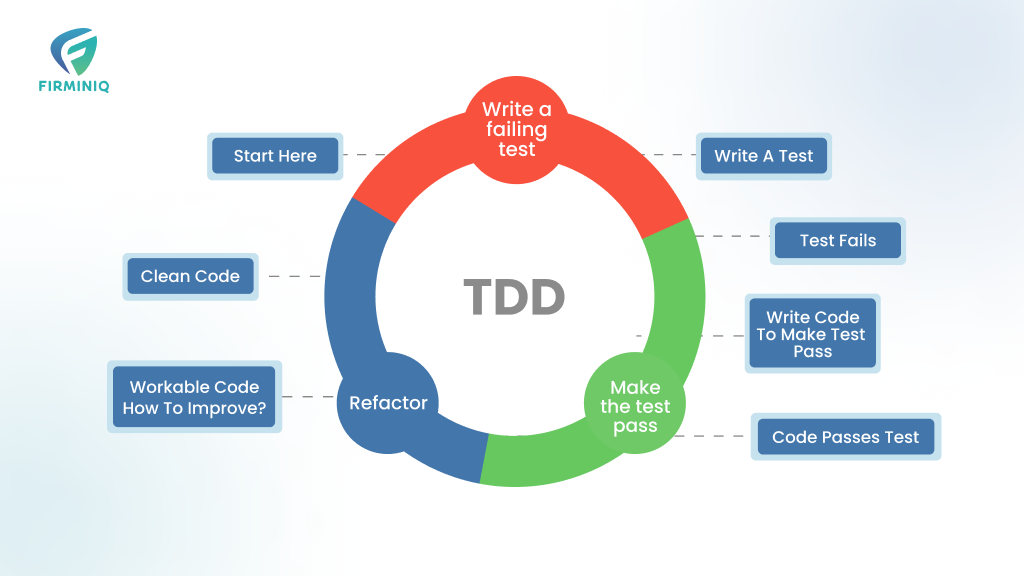
\includegraphics[width=0.8\textwidth]{Figuras/TDD.png}
    \legend{Fonte: \citeonline{firminiq2024}.}
\end{figure}

Mais do que uma simples técnica de verificação, o TDD é uma poderosa ferramenta de \textit{design} de software. Ao escrever o teste primeiro, o desenvolvedor atua como o primeiro cliente do próprio código, o que o obriga a pensar na interface pública da classe, em suas dependências e em sua responsabilidade. Dificuldades na escrita de um teste, como a necessidade de configurações complexas ou o uso excessivo de dependências simuladas (\textit{mock objects}), são indícios claros de problemas arquiteturais, denunciando alto acoplamento e baixa coesão estrutural \cite{martin_clean,aniche2012}. %

Para maximizar a eficiência de execução e manutenção, a estratégia de testes de um sistema deve ser distribuída em diferentes níveis de granularidade, conceito frequentemente ilustrado pela Pirâmide de Testes. A base da pirâmide é composta pelos testes de unidade, que são extremamente rápidos, isolados e verificam o comportamento de pequenas partes do código, como classes ou métodos específicos. O nível intermediário abriga os testes de integração, responsáveis por garantir a correta comunicação entre os componentes internos e sistemas de infraestrutura externos, como bancos de dados ou serviços de terceiros. No topo da pirâmide estão os testes de ponta a ponta (\textit{end-to-end}) e de aceitação, que validam o sistema inteiro através da interface com o usuário, simulando o comportamento real da aplicação de forma mais custosa e lenta \cite{aniche2012,silveira2012}. %

Por fim, do ponto de vista arquitetural, os testes devem ser tratados como componentes essenciais do sistema. Contudo, para que não se tornem frágeis e difíceis de manter, eles devem ser desacoplados de elementos voláteis, como a Interface de Usuário (UI) ou as ferramentas de persistência. Uma arquitetura limpa e bem projetada permite que as regras de negócio centrais sejam exaustivamente testadas de forma isolada, garantindo execuções rápidas e \textit{feedback} imediato para a equipe de desenvolvimento \cite{martin_clean}. %

\subsection{Arquitetura Limpa e Separação de Responsabilidades}

O projeto arquitetural do sistema foi concebido sob a ótica da Separação de Responsabilidades (\textit{Separation of Concerns} - SoC), dividindo o software em camadas isoladas com papéis independentes e bem definidos. A interface de usuário no \textit{front-end} foca exclusivamente na experiência de uso e integração visual, enquanto a lógica de execução do negócio permanece no \textit{back-end}. Isso respeita a premissa fundamental da Arquitetura Limpa de que as regras centrais da aplicação jamais devem depender de detalhes periféricos de entrega, considerando que a tecnologia \textit{Web} ou a interface de usuário são apenas detalhes de implementação \cite{martin_clean}.

No que tange à camada de dados, a persistência foi totalmente abstraída por meio de ferramentas de Mapeamento Objeto-Relacional (ORMs, como \textit{Prisma} e \textit{SQLAlchemy}). O uso de ORMs atua como uma ponte que suaviza a discrepância entre o paradigma relacional e o orientado a objetos, mitigando a dependência direta de consultas SQL. Essa prática garante que o banco de dados seja tratado estritamente como um detalhe de infraestrutura de baixo nível, impedindo que sua estrutura tabular polua a lógica central e as regras de negócio do domínio \cite{martin_clean,silveira2012}.

Por fim, a maturidade da arquitetura expressa-se também pela adoção de Padrões de Projeto (\textit{Design Patterns}) na construção do compilador. O uso do padrão \textit{Factory}, por exemplo, foi empregado para encapsular a lógica complexa de instanciação dos componentes de análise (\textit{Lexer} e \textit{Scanners}). Essa abordagem centraliza a decisão de criação de objetos, favorecendo a coesão e reduzindo drasticamente o acoplamento global do sistema \cite{silveira2012}.

\subsection{Qualidade de Código e \textit{Clean Code}}

A construção de um software ágil e sustentável esbarra invariavelmente na qualidade de sua base de código. O código-fonte é a linguagem formal na qual os requisitos de um sistema são expressos e detalhados de modo que a máquina possa executá-los. No entanto, sob a pressão de prazos, é comum que as equipes produzam códigos desorganizados, resultando em uma degradação estrutural contínua que, a longo prazo, faz a produtividade despencar, podendo até mesmo inviabilizar a evolução do projeto \cite{martin_clean_code}.

Para combater essa entropia, a adoção das práticas de Código Limpo torna-se essencial. A escrita de um código limpo exige disciplina, o uso consciente de padrões e uma sensibilidade aguçada para reconhecer a desorganização e aplicar refatorações. Um código limpo deve ser elegante, simples, direto e, sobretudo, legível para os seres humanos. O profissionalismo no desenvolvimento de software pressupõe que o código não deve apenas funcionar, mas deve ser fácil de entender, alterar e estender por outros desenvolvedores \cite{martin_clean_code}.

Dentre as diretrizes estruturais básicas e inegociáveis para a manutenção dessa clareza na base de código, destacam-se:

\begin{itemize}
    \item \textbf{Nomes Significativos:} A nomenclatura de variáveis, funções, parâmetros e classes deve revelar claramente a sua intenção e responder ao porquê de sua existência e ao que o componente faz. Deve-se evitar o uso de siglas obscuras, codificações desnecessárias ou trocadilhos que exijam mapeamentos mentais, facilitando assim a leitura fluida e a busca no código.

    \item \textbf{Funções Pequenas e Focadas:} Uma função deve ser extremamente concisa e projetada para fazer estritamente uma única coisa, mantendo um único nível de abstração. Funções extensas que realizam múltiplas tarefas, agrupam várias seções lógicas ou que misturam tratamento de erros com a lógica de negócio violam a organização e dificultam o entendimento e a testabilidade.

    \item \textbf{Uso Consciente de Comentários:} O uso de comentários costuma compensar a incapacidade do programador de se expressar claramente através do próprio código. Eles não devem ser utilizados para encobrir ou justificar um código ruim ou confuso. A energia da equipe deve ser direcionada para tornar o código tão claro e autoexplicativo que elimine a necessidade de anotações redundantes.

    \item \textbf{Eliminação de Duplicidade e Refatoração contínua:} A repetição de código é o grande inimigo de um sistema bem desenvolvido, pois representa trabalho, risco e complexidade desnecessária. Deve-se melhorar o design do código de forma contínua, aplicando refatorações que tornem o sistema mais enxuto e compreensível, sem alterar o seu comportamento externo \cite{martin_clean_code}.
\end{itemize}

\subsection{FastAPI: Framework para APIs de Alto Desempenho}

O FastAPI é um \textit{framework} web moderno e de alto desempenho projetado para a construção de Interfaces de Programação de Aplicações (APIs) utilizando a linguagem Python. Sua arquitetura foi desenhada para ser simples, rápida e eficiente, tirando proveito das funcionalidades modernas da linguagem, como as anotações de tipo explícitas (\textit{type hints}) e o suporte nativo a operações da programação assíncrona \cite{fastapi2026}.

Um dos pilares que garantem a alta performance do FastAPI é a sua fundação sobre a especificação ASGI (\textit{Asynchronous Server Gateway Interface}) e o \textit{framework} Starlette. Diferentemente de \textit{frameworks} web tradicionais que utilizam o modelo síncrono (WSGI), a arquitetura assíncrona do FastAPI permite que o servidor gerencie milhares de conexões simultâneas de forma eficiente, processando operações de entrada e saída (I/O) sem bloquear a \textit{thread} de execução. Em ambientes de produção, aliado a servidores de aplicação como o Uvicorn, o FastAPI é capaz de suportar picos de mais de 20.000 requisições por segundo, apresentando desempenho comparável a linguagens compiladas como Go e plataformas como o NodeJS \cite{dasroot2026}.

Outra característica central do \textit{framework} é a integração profunda com a biblioteca Pydantic, que assume a responsabilidade pela validação e serialização rigorosa dos dados. Ao invés de exigir a aprendizagem de uma nova micro-linguagem de validação, o desenvolvedor utiliza os tipos de dados padrão do próprio Python. A ferramenta converte automaticamente os dados de entrada (como o corpo de uma requisição em formato JSON) para os tipos corretos e gera mensagens de erro estruturadas e detalhadas caso a validação falhe, garantindo uma maior segurança e consistência no processamento \cite{fastapi2026,dunossauro2026}.

Além disso, a plataforma é construída estritamente em torno de padrões abertos, notadamente a especificação OpenAPI e o JSON Schema. Essa aderência aos padrões permite que o FastAPI gere de forma automática e dinâmica a documentação interativa da API, disponibilizando interfaces prontas para o consumo do desenvolvedor, como o Swagger UI e o ReDoc. Isso reduz drasticamente o tempo gasto com a documentação manual, facilita a integração com sistemas de \textit{front-end} e permite a geração automática de clientes (\textit{SDKs}) em diversas linguagens \cite{fastapi2026}.

Por fim, o \textit{framework} incorpora um sistema de Injeção de Dependência poderoso, porém intuitivo, que simplifica a integração do código da aplicação com bancos de dados relacionais (através de ORMs como o SQLAlchemy), além de prover mecanismos nativos e facilitados para a implementação de segurança e autenticação, como fluxos OAuth2 e \textit{tokens} JWT. Toda essa gama de funcionalidades faz do FastAPI uma escolha robusta, tanto para a criação rápida de protótipos quanto para sistemas corporativos altamente escaláveis \cite{dunossauro2026}.

\section{Softwares Educativos e Tecnologias de Apoio à Aprendizagem}

Uma plataforma educativa é um ambiente virtual desenvolvido para apoiar processos de ensino e aprendizagem, oferecendo recursos, ferramentas e conteúdos que facilitam a interação entre alunos, professores e instituições de ensino. Nesse cenário de transformação, a escolha da ferramenta certa não é apenas uma questão tecnológica, mas um fator determinante para o engajamento, a motivação e o sucesso educacional \cite{benedetti2025}.

Contudo, para aproveitar o potencial das novas tecnologias, a instituição de ensino precisa ir além da simples adoção de ferramentas digitais. É essencial entender o propósito pedagógico por trás de cada inovação, garantindo que a tecnologia esteja sempre a serviço da aprendizagem e não o contrário. Afinal, a tecnologia educacional atua como um meio que exige professores preparados para usar recursos digitais de forma criativa e estratégica, conectando os alunos a um aprendizado relevante, dinâmico e significativo \cite{mindmakers2025}.

Quando projetada com esse foco pedagógico, uma plataforma educativa bem estruturada permite a personalização do aprendizado, ajustando-se ao ritmo e ao estilo de cada aluno, o que maximiza seu potencial e promove uma assimilação muito mais eficaz do conteúdo. Essa abordagem valoriza o tempo de cada estudante e amplia as suas capacidades ao longo de toda a jornada educacional. Além disso, a integração de dinâmicas interativas nas ferramentas de ensino, como a gamificação e a aprendizagem baseada em desafios, transforma a educação em um processo envolvente de recompensas. Esses sistemas lúdicos ajudam a despertar o interesse contínuo dos alunos e a desenvolver habilidades socioemocionais indispensáveis, como persistência e colaboração \cite{benedetti2025,mindmakers2025}.


\label{sec:softwares-apoio}
 


\section{Trabalhos Relacionados}
\label{sec:trabalhos-relacionados}

Esta seção analisa ferramentas e linguagens que compartilham objetivos com a solução proposta, seja no apoio ao ensino de programação, seja na construção de compiladores para fins didáticos. O critério de seleção dos trabalhos aqui analisados, baseado na representatividade dos dois eixos do problema, está descrito na Seção~\ref{sec:selecao-trabalhos}. Os trabalhos estão organizados nas duas subseções seguintes conforme o eixo a que pertencem: de um lado, os ambientes voltados à iniciação em programação; de outro, os projetos didáticos de construção de compiladores. Cada trabalho é descrito quanto à sua proposta, às suas características e às suas limitações; ao final, uma análise crítica consolida a comparação e evidencia o diferencial da plataforma desenvolvida frente ao estado da arte.

\subsection{Ambientes Voltados à Iniciação em Programação}

Reúnem-se aqui as ferramentas cujo público-alvo é o estudante em primeiro contato com a programação e cujo propósito declarado é reduzir o atrito desse contato inicial. Cada uma é examinada segundo os três eixos anunciados no início desta seção: as escolhas de interface, os recursos pedagógicos e as estratégias de interação com o estudante.

\noindent\textbf{Portugol Studio e Portugol Webstudio}

\textit{Escolhas de interface.} O Portugol Studio é um Ambiente de Desenvolvimento Integrado (IDE) educacional de código aberto, projetado e mantido pelo Laboratório de Inovação Tecnológica na Educação (LITE) da UNIVALI, cuja composição de tela abstrai a complexidade dos ambientes profissionais sem abandonar sua organização geral. Visando reduzir barreiras tecnológicas, o projeto evoluiu para o Portugol Webstudio, versão que permite compilar e executar códigos diretamente no navegador, dispensando qualquer instalação no computador do usuário \cite{univali2026,martins2025}.

\textit{Recursos pedagógicos.} O recurso central é a linguagem Portugol, com sintaxe baseada em C e PHP, porém com comandos totalmente estruturados na língua portuguesa, o que elimina a exigência de operar em dois idiomas simultaneamente. A esse núcleo somam-se recursos didáticos de visualização: execução passo a passo por meio de depurador, inspetor de variáveis em tempo real e árvore estrutural do código, que tornam observável o comportamento interno da máquina \cite{univali2026,gomes2020}.

\textit{Estratégias de interação.} A interação apoia-se no acompanhamento visual da execução, permitindo ao estudante confrontar o algoritmo imaginado com o efetivamente executado. O suporte nativo a bibliotecas gráficas e de som amplia essa estratégia ao viabilizar a criação de jogos com interface gráfica, cuja saída fornece retorno imediato e concreto sobre o efeito do código escrito \cite{gomes2020,martins2025}.

% -------------------------------------------------------------------------------------------------------------

\noindent\textbf{Quorum: linguagem de programação baseada em evidências}

\textit{Escolhas de interface.} A equipe do projeto desenvolveu o Quorum Studio, um Ambiente de Desenvolvimento Integrado nativamente acessível, isto é, concebido desde o início para operar com leitores de tela, e não adaptado a eles posteriormente. A infraestrutura é flexível: a linguagem executa tanto \textit{offline}, gerando \textit{bytecode} para a Máquina Virtual Java, quanto diretamente no navegador do usuário \cite{ladner2019,quorum2025}.

\textit{Recursos pedagógicos.} A linguagem Quorum foi inicialmente concebida pelo pesquisador Andreas Stefik com o objetivo de ser nativamente acessível a estudantes cegos ou com deficiência visual, e evoluiu para uma linguagem de propósito geral mantendo sua premissa principal: ser orientada a evidências. Suas regras sintáticas e semânticas não decorrem de tradição ou intuição, mas de ensaios controlados com usuários novatos e experientes. Os experimentos compararam o desempenho de novatos em linguagens comerciais com o obtido em uma linguagem de controle cujas palavras-chave foram geradas aleatoriamente, isolando o efeito da forma sintática. Os resultados indicaram que remover símbolos obscuros --- chaves, colchetes e pontos e vírgulas --- e substituí-los por palavras de uso comum reduz consistentemente as taxas de erro sintático, o que se materializa em construções como \texttt{repeat 10 times} \cite{stefik2013}.

\textit{Estratégias de interação.} A modalidade primária de interação prevista é auditiva: a linguagem foi projetada para que sua leitura por síntese de voz permaneça clara, exigência que condiciona desde a escolha das palavras-chave até a pontuação. O ecossistema estende essa interação a domínios de saída variados, suportando desde lógicas simples até jogos, processamento de áudio e robótica, o que oferece formas de perceber o resultado do programa que não dependem exclusivamente da leitura visual \cite{ladner2019,quorum2025}.

\noindent\textbf{Beecrowd: prática de algoritmos e avaliação automatizada}

\textit{Escolhas de interface.} O Beecrowd, anteriormente conhecido como URI Online Judge, é uma plataforma \textit{online} organizada em torno de um acervo navegável por categorias e níveis de dificuldade. A interface não oferece ambiente de desenvolvimento: o estudante redige a solução em ferramenta externa e submete o código pronto, o que pressupõe um ambiente já configurado \cite{garcia2024}.

\textit{Recursos pedagógicos.} O acervo conta com milhares de desafios algorítmicos, das lógicas fundamentais às estruturas de dados complexas, e admite submissões em diversas linguagens de mercado, como C++, Python, Java e JavaScript. A graduação de dificuldade é o principal recurso didático, pois permite progressão por incrementos e seleção, pelo professor, de conjuntos coerentes com o momento da disciplina \cite{garcia2024,ferreira2025}.

\textit{Estratégias de interação.} A característica definidora é o sistema de juiz \textit{online}: o aluno lê a especificação do problema, desenvolve o código e o submete; em segundos, o sistema compila, executa e testa a solução contra casos de teste fechados, devolvendo vereditos como ``\textit{Accepted}'', ``\textit{Wrong Answer}'' ou ``\textit{Presentation Error}''. Cabe observar que esse retorno informa o resultado, mas não localiza o erro no código. Aliada a elementos de gamificação como fóruns e \textit{rankings}, a validação em tempo real estimula a prática contínua e desloca o aluno de uma posição passiva para a resolução ativa de problemas \cite{ferreira2025,maonocodigo2022}.

\subsection{Projetos Didáticos de Construção de Compiladores}

Reúnem-se aqui as iniciativas voltadas ao ensino da construção de tradutores. Embora se dirijam a um público mais avançado, suas decisões técnicas e pedagógicas dialogam diretamente com o núcleo de tradução que sustenta a plataforma proposta, e por isso são examinadas segundo os mesmos três eixos.

\noindent\textbf{Laila: gerador de analisadores léxicos e sintáticos \textit{online}}

\textit{Escolhas de interface.} A ferramenta oferece um ambiente de desenvolvimento integrado totalmente \textit{online}. O módulo de interação com o usuário foi construído em JavaScript com o \textit{framework} VueJS e a biblioteca CodeMirror, garantindo edição de código com destaque de sintaxe e identificação de erros em tempo real; o processamento ocorre por meio de uma API REST em Python, que executa FLEX e Bison no servidor, captura falhas como laços infinitos ou erros de compilação e devolve as saídas ao navegador. A escolha responde a um obstáculo concreto: o ensino prático da disciplina exige a instalação e a configuração de ferramentas como GCC, FLEX e Bison, tarefas árduas em sistemas operacionais não baseados em Linux \cite{ladgelson2021}.

\textit{Recursos pedagógicos.} O recurso didático central é permitir que o aluno projete, escreva e teste seus analisadores léxicos e sintáticos sem qualquer configuração local, concentrando o tempo de laboratório no objeto de estudo e não em sua preparação \cite{ladgelson2021}.

\textit{Estratégias de interação.} A interação organiza-se em um ciclo curto entre edição, submissão e retorno do resultado. Em estudos de caso realizados com turmas de Ciência da Computação, os participantes relataram melhoria na compreensão dos algoritmos de análise léxica e sintática, atribuída à praticidade de testar as linguagens em tempo real, e o uso da plataforma contornou os problemas de compatibilidade de ambiente \cite{ladgelson2021}.

\noindent\textbf{\textit{chibicc}: abordagem incremental para o ensino de compiladores}

\textit{Escolhas de interface.} Este é o caso em que a análise por eixos revela a maior distância em relação às demais ferramentas: o \textit{chibicc} não possui interface própria. Trata-se de um repositório de código-fonte, cuja fruição pressupõe editor, cadeia de compilação e sistema de controle de versão já instalados e dominados pelo estudante. Toda a mediação recai sobre o histórico de \textit{commits} do projeto \cite{ueyama2020}.

\textit{Recursos pedagógicos.} O diferencial pedagógico reside na abordagem incremental. Em vez de apresentar uma arquitetura monolítica desde o início, o projeto orienta a construção do compilador passo a passo: o aluno começa por um tradutor rudimentar, capaz de aceitar apenas um único número como linguagem válida, e a partir dessa base mínima acrescenta, de forma isolada a cada etapa, novos recursos gramaticais e semânticos, até que a linguagem aceita corresponda à especificação do C11. Apesar do enfoque educacional, o resultado suporta ampla variedade de recursos dessa especificação, sendo capaz de compilar sem modificações programas de grande porte, como o sistema de controle de versão Git e o banco de dados SQLite \cite{ueyama2020}.

\textit{Estratégias de interação.} Não há retorno automatizado nem execução assistida: a interação consiste na leitura do código de cada etapa e em sua reimplementação pelo estudante, que verifica o próprio progresso executando manualmente a suíte de testes do projeto. O método desmistifica a transição do código-fonte para o código de máquina, mas transfere integralmente ao aprendiz a responsabilidade pela regulação do próprio ritmo \cite{ueyama2020}.

\subsection{Análise Crítica e o Diferencial da Solução Proposta}

A Tabela~\ref{tab:comparativo} sintetiza as ferramentas examinadas segundo os três eixos adotados nesta seção, acrescentando a coluna que expressa o traço distintivo da proposta: a possibilidade de o próprio estudante redefinir a sintaxe da linguagem.

\begin{landscape}
\begin{table}[p]
    \centering
    \caption{Comparativo entre as ferramentas analisadas e a plataforma proposta, segundo os três eixos de análise.}
    \label{tab:comparativo}
    \footnotesize
    \setlength{\tabcolsep}{4pt}
    \renewcommand{\arraystretch}{1.3}
    \begin{tabular}{|>{\raggedright\arraybackslash}p{2.3cm}|>{\raggedright\arraybackslash}p{4.3cm}|>{\raggedright\arraybackslash}p{4.7cm}|>{\raggedright\arraybackslash}p{4.7cm}|>{\raggedright\arraybackslash}p{4.4cm}|}
        \hline
        \textbf{Ferramenta} & \textbf{Escolhas de interface} & \textbf{Recursos pedagógicos} & \textbf{Estratégias de interação} & \textbf{Personalização da sintaxe pelo estudante} \\
        \hline
        Portugol Studio e Webstudio
          & IDE própria, em versão local e em versão executada no navegador
          & Linguagem com palavras-chave em português; depurador, inspetor de variáveis e árvore sintática
          & Acompanhamento visual da execução; projetos gráficos e sonoros
          & Não \\
        \hline
        Quorum
          & IDE própria concebida para leitores de tela; execução local ou no navegador
          & Sintaxe definida por evidência empírica; operadores expressos por palavras
          & Leitura por síntese de voz; saídas em áudio, gráficos e robótica
          & Não \\
        \hline
        Beecrowd
          & Plataforma web sem ambiente de edição; exige ferramenta externa
          & Acervo graduado por tema e dificuldade; múltiplas linguagens de mercado
          & Ciclo submissão--veredito, sem localização do erro; gamificação
          & Não \\
        \hline
        Laila
          & IDE web com destaque de sintaxe e diagnóstico \textit{inline}
          & Dispensa a instalação de FLEX, Bison e GCC, liberando o tempo de laboratório
          & Ciclo curto entre edição, execução e diagnóstico
          & Sim, mas como objeto de estudo: o aluno escreve gramáticas formais \\
        \hline
        \textit{chibicc}
          & Sem interface própria; repositório de código-fonte
          & Trajetória incremental, uma capacidade da linguagem por etapa
          & Leitura e reimplementação do código; sem retorno automatizado
          & Não \\
        \hline
        \textbf{Plataforma proposta}
          & IDE web própria, com terminal integrado e sistema de arquivos
          & Exposição das fases de tradução (\textit{tokens} e código intermediário); avaliação automatizada de exercícios
          & Execução e depuração passo a passo; erros relatados no vocabulário escolhido pelo próprio estudante
          & Sim: palavras-chave, delimitadores de bloco, operadores, literais booleanos e terminador de instrução \\
        \hline
    \end{tabular}
    \legend{Fonte: elaborado pelo autor.}
\end{table}
\end{landscape}

Ao observar o estado da arte das ferramentas de apoio ao ensino de programação e de compiladores, nota-se que as soluções existentes tendem a seguir dois caminhos distintos, ambos com limitações estruturais significativas para o aluno iniciante. O primeiro caminho é o das ferramentas com foco em lógica e prática contínua, como o Portugol Studio, a linguagem Quorum e a plataforma Beecrowd. Embora o Quorum comprove cientificamente que a sintaxe tradicional é uma barreira real de aprendizado \cite{stefik2013} e o Portugol traduza os comandos para a língua nativa, todas essas plataformas compartilham um obstáculo comum: a imposição de uma gramática estática e rigorosa. O aluno continua obrigado a memorizar palavras-chave fixas e a se adequar a avaliadores automáticos inflexíveis, que rejeitam lógicas corretas devido a erros mínimos de formatação ou digitação.

O segundo caminho engloba as ferramentas criadas especificamente para o ensino prático da disciplina de compiladores, como a plataforma Laila e o projeto \textit{chibicc}. Apesar de serem soluções de excelência em seus respectivos nichos seja abstraindo configurações de ambiente por meio de plataformas web, ou ensinando a construção incremental de um tradutor, elas possuem um enfoque estritamente sistêmico e de baixo nível. São metodologias voltadas para alunos avançados de Ciência da Computação, exigindo o domínio prévio de linguagens complexas (como C11) e de ferramentas geradoras pesadas (como FLEX e Bison), o que as torna inadequadas para a quebra da barreira linguística introdutória.

É exatamente na intersecção e na superação dessas lacunas que o presente projeto se destaca de forma inovadora. O interpretador dinâmico construído neste trabalho desloca toda a complexidade arquitetural da análise léxica e sintática para os bastidores, oferecendo uma IDE web focada inteiramente na flexibilidade cognitiva do usuário iniciante. Em vez de impor uma ``sintaxe ideal única'' ou de focar no mapeamento de instruções para o \textit{hardware}, a plataforma delega a criação estrutural da linguagem ao próprio estudante.

Ao permitir que o aluno personalize as palavras-chave, os operadores e as regras estruturais de sua própria linguagem de forma dinâmica no navegador, o sistema atua como um laboratório seguro de experimentação algorítmica. Essa abordagem suprime a necessidade de adaptação imediata a um idioma comercial fixo, mitigando drasticamente a carga cognitiva e a frustração atrelada aos erros gramaticais. Dessa forma, o software proposto consolida-se não apenas como um ambiente de execução, mas como uma ponte pedagógica: uma ferramenta que prioriza a estrutura do pensamento computacional e suaviza a curva de aprendizado, preparando o estudante com muito mais confiança antes de sua transição para as linguagens estritas e juízes online do mercado de software.


